\section{Computational evidence}\label{sec:computational}

The computations ask whether complete-fleet convexification can be bounded at a changed supply market, and which parts of repeated optimization remain costly.  They do not estimate a population-level speedup.  We use two deliberately small synthetic cases and two depot variants of a single 37-service Hildenbrand timetable.  Depot 15 and depot 16 use different depots in that base network; they are not independent public replications.  The reported results come from one run of each campaign.  The campaigns reuse cases, code paths, and in some instances source-plan evidence, so their cells cannot be pooled as independent trials.

For a case $I$, let $\mathcal F(I)$ be its set of \emph{complete} physically feasible fleet schedules.  A column $x\in\mathcal F(I)$ includes the service assignment, vehicle paths, charging decisions, and full-horizon load $e(x)$, with operating cost $c(x)$.  For the separable quadratic supply model
\begin{equation}\label{eq:computational-supply}
 G_s(e)=\sum_{t=1}^{T}\left(a_{s,t}e_t+\tfrac12 b_t e_t^2\right),\qquad s\in\{0,1\},
\end{equation}
the pure-fleet and complete-fleet-hull objectives are
\begin{equation}\label{eq:computational-D-CH}
\begin{aligned}
 D_s&=\min_{x\in\mathcal F(I)}\{c(x)+G_s(e(x))\},\\
 CH_s&=\min_{(e,c)\in\operatorname{conv}\{(e(x),c(x)):x\in\mathcal F(I)\}}\{c+G_s(e)\}.
\end{aligned}
\end{equation}
State 0 is the source market and state 1 is the changed target market on the \emph{same} physical case.  In the public cases $T=30$, $b_t=1/900$, and $a_{0,t}=0.20$ throughout; the target has $a_{1,t}=0.18$ in the first 15 periods and $0.22$ in the last 15.  The synthetic cases have four periods and similarly paired source and target coefficients.  This controlled price change makes same-case reuse meaningful without treating a source-market solution as a target-market optimum.

We report an interval $[L,U]$ for $CH_1$ only when the run produced the required evidence.  Its upper endpoint is the objective of a feasible \emph{convex mixture} of complete fleet columns.  That mixture is a valid hull point, but generally cannot be dispatched as one fleet schedule.  A global lower endpoint is assembled from physical fleet-pricing evidence in the target market, including checked inherited physical-pricing bounds where explicitly indicated.  Native mixed-integer solver bounds and replayed numerical solutions retain the solver's tolerance qualifications; they are computational enclosures, not exact proofs for the ideal model.  A zero or small gap in the finite \emph{restricted} column pool does not close the global interval: ungenerated complete fleets still matter.  Nor does an interval for $CH_1$ alone establish the pure-fleet value $D_1$, a nonconvexity gap $D_1-CH_1$, or support by any proposed tariff.

\begin{table}[t]
\centering\small
\caption{Development campaigns and their declared scope.  Outcomes count cells for the two iterative-hull campaigns and fixed-price calls for the pricing-start campaign.  The same four physical cases recur across campaigns.}\label{tab:computational-scope}
\begin{tabular}{>{\raggedright\arraybackslash}p{0.20\linewidth}>{\raggedright\arraybackslash}p{0.35\linewidth}>{\raggedright\arraybackslash}p{0.36\linewidth}}
\toprule
Campaign & Design & Observed outcomes \\
\midrule
Feasible-pool pilot & Three hull methods $\times$ four cases $\times$ two markets; reserve and source-column reuse & 24 cells: 7 certified and 17 budget-exhausted.  Both public target depot variants remained open. \\
Solver-baseline comparison & Four ordered hull methods $\times$ four cases $\times$ two markets; numerical restricted master and physical-bound cache & 32 cells: 11 certified, 18 budget-exhausted, 3 failed.  No public target cell certified. \\
Pricing-start pilot & Cold versus submitted movement start at two fixed price queries on four cases & 16 calls returned.  Four synthetic pairs agreed within tolerance; all eight public calls reached the native 160-s cap. \\
\bottomrule
\end{tabular}
\end{table}

\subsection{Complete-fleet hull updates}

The first pilot compared a legacy cold run, a cold run that reserves time for a subsequent restricted master, and that reserve policy with feasible source-column reuse.  The reserve made a second master possible in all four public reserve-cold cells, while the corresponding legacy cells ended after one master.  In the changed market, the reuse method admitted two feasible state-0 columns to its first master, obtained one fresh target-market priced column, and processed it in a second master.  The source columns help form target-market feasible mixtures, but they do not replace target-market pricing for a global lower bound.

On the synthetic cyclic case, all six market-by-method cells certified.  On the multivisit case, the source market exhausted its budget in all three methods.  In the target market, reuse closed the global enclosure while the two cold methods exhausted their budgets: its displayed interval is $[84.72,84.73]$ after outward rounding, versus $[81.17,86.05]$ for reserve cold.  This is a diagnostic of the method under the declared small-case budget, not a claim about larger networks.

For the public target cases, reserve cold lowered the feasible upper relative to legacy cold, from $547.47$ to $526.31$ at depot 15 and from $549.70$ to $531.90$ at depot 16.  Reuse lowered those upper endpoints further to $469.89$ and $490.67$.  Yet its fresh global lower endpoints were $315.76$ and $329.22$, below reserve cold's $339.35$ and $377.65$.  Thus the upper improvements of $56.43$ and $41.24$ do not imply tighter \emph{global} enclosures; in depot 16 the interval width actually grows.  The public reuse cells stopped at projected rational-polishing bit growth, whereas reserve-cold cells stopped at the explicit pricing-reserve guard.

The ordered solver-baseline comparison then retained feasible columns and introduced two further mechanisms.  A numerical quadratic-program (QP) \emph{restricted-master proposal} selects mixture weights over the currently known complete-fleet columns; a checked rational replay admits its objective and residual.  The fourth method also re-evaluates an inherited \emph{physical-pricing lower bound} under the changed market's Fenchel conjugate.  This cache concerns already-checked physical pricing evidence, not a cache of an unverified schedule or a substitute for all fresh target-market pricing.  Table~\ref{tab:public-hull} gives all public target outcomes in this comparison, including the paid source-state work and source-admission cost for retained methods.

\begin{table}[t]
\centering\small
\caption{Public target-market hull evidence in the ordered solver-baseline comparison.  $L$ is rounded down and $U$ up to two decimals; unrounded stored values determine certification.  ``Exhausted'' means budget exhausted.  Paid time includes both market states and, where applicable, parent source admission.  A failed target has no final interval even though its time was paid.}\label{tab:public-hull}
\begin{tabular}{llrrrr}
\toprule
Depot & Method & $L$ & $U$ & Paid (s) & Outcome \\
\midrule
15 & Reserve cold & --- & --- & 347.20 & failed \\
15 & Reserve + pool & 315.76 & 469.89 & 354.61 & exhausted \\
15 & QP + pool & --- & --- & 349.88 & failed \\
15 & QP + pool + cache & 405.83 & 471.52 & 352.27 & exhausted \\
\addlinespace
16 & Reserve cold & 377.65 & 531.90 & 351.08 & exhausted \\
16 & Reserve + pool & 350.87 & 490.67 & 353.48 & exhausted \\
16 & QP + pool & --- & --- & 349.53 & failed \\
16 & QP + pool + cache & 420.45 & 491.46 & 352.22 & exhausted \\
\bottomrule
\end{tabular}
\end{table}

\begin{figure}[t]
\centering
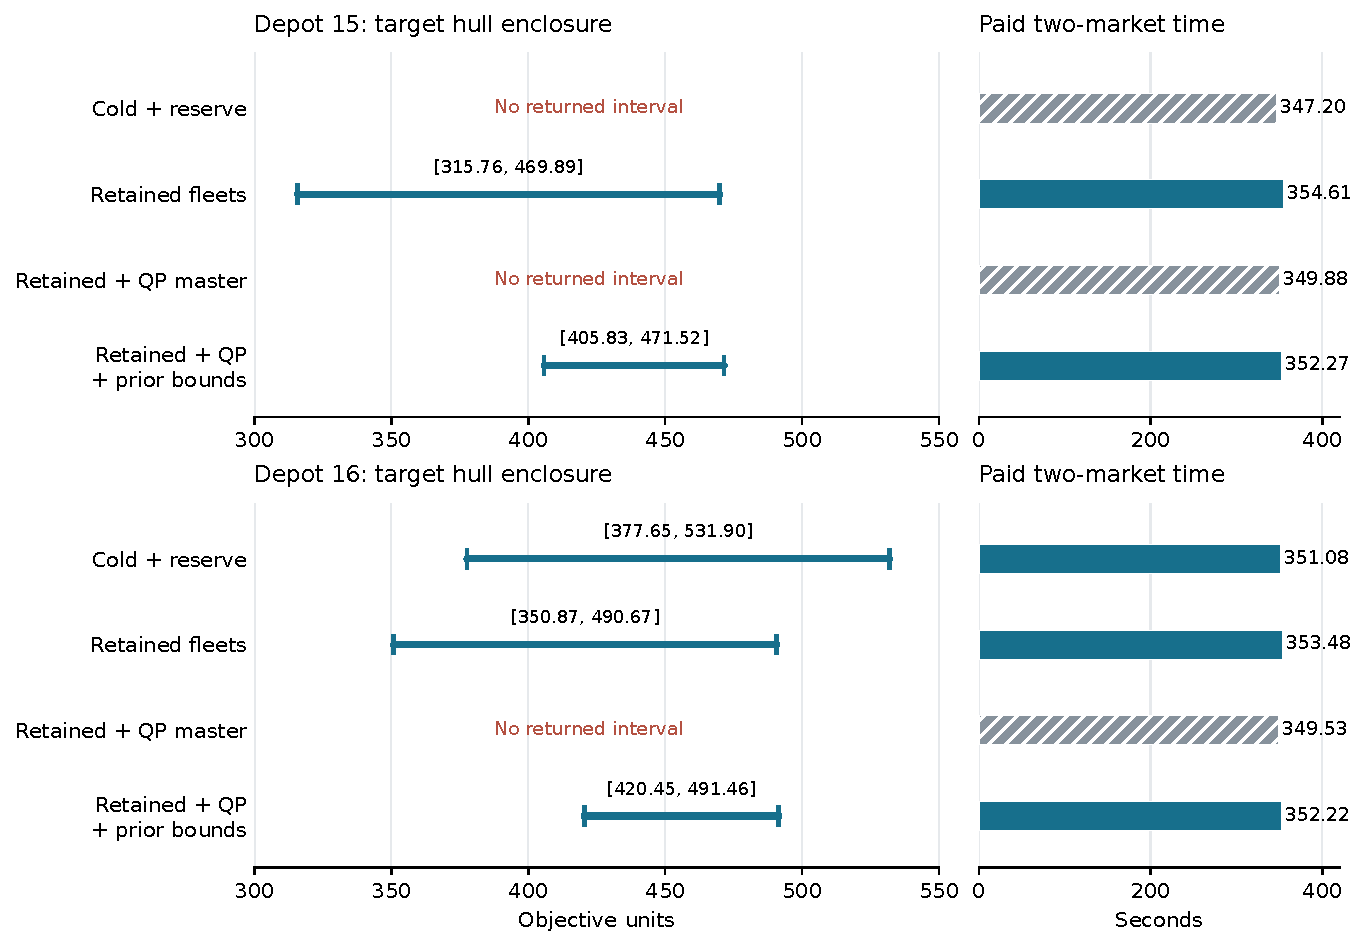
\includegraphics[width=\linewidth]{figures/public_hull_comparison.pdf}
\caption{All eight public target cells in the ordered solver-baseline comparison: global hull intervals and paid two-market cost.  Lower endpoints use physical-pricing evidence and upper endpoints feasible mixtures.  Every completed interval remains open.  Hatching marks a failed target with no final bound interval; its spent time remains in the paid-cost panel.  The depot variants share one timetable.}\label{fig:public-hull}
\end{figure}

The completed public QP-and-cache cells ended with restricted-pool residuals below the configured $10^{-6}$ pool tolerance, without exhausting the rational-polishing bit budget.  Their \emph{global} intervals were still open by $65.68$ and $71.00$ objective units, and both stopped on native remaining-time budget.  In each, one fresh physical target pricing result was recorded.  The inherited, target-revalued physical lower exceeded the best fresh lower within the same run by $98.82$ at depot 15 and $69.83$ at depot 16; the selected global lowers were $405.83$ and $420.45$.  This within-run decomposition identifies a useful source of bound strength.  It cannot isolate a causal cache effect across methods: the QP-without-cache target cells failed, and the cached method also incurs source-state computation and admission work.

An implementation error when a pricing call returned no incumbent caused three target failures: depot 15 reserve cold and both depot variants with the numerical restricted master and pool but no bound cache.  No new completed pricing result or global bound was produced for the failing call.  Their spent time remains in Table~\ref{tab:public-hull}, and their missing intervals cannot be imputed from another method.  On the two synthetic cases, all methods certified cyclic in both markets, while the three retained-pool methods certified multivisit in the changed market and reserve cold did not.

The iterative timings explain why a faster restricted master alone would have limited impact on these public cells.  Recorded successful public physical-pricing calls were about 160~s, while QP proposal took $0.77$--$1.07$~s and rational replay $0.51$--$0.53$~s in the completed cached targets.  The feasible-pool pilot's public changed-market pricing consumed roughly 160--172~s per cell; its master native solves were below $0.01$~s, though rational polishing in reuse took about six seconds.  Component scopes differ and may overlap, so these quantities are not an additive time budget.  In the first pilot, paid source-plus-target times were about 369~s for legacy cold, 350~s for reserve cold, and 351--352~s for reuse on the public variants.  Those methods ended at different bounds and stopping points.  Neither campaign specified an equal-quality time target, and none of these differences is an equal-quality speedup estimate.

\subsection{Fixed-price movement starts}

The separate pricing-start pilot probes the physical pricing oracle at fixed prices rather than running the iterative hull.  Its \emph{linear} query uses the target market's coefficients $p_t=a_{1,t}$.  Its \emph{marginal} query uses $p_t=a_{1,t}+b_te_t(\bar x)$, where $\bar x$ is the cheapest linear-bill schedule among the common feasible source columns.  This anchor is a selected feasible column, not a certified target planner optimum.  The two price vectors are distinct in all four cases.  A common feasible source schedule supplied a baseline upper to both arms; the start arm additionally submitted its checked discrete movement selections to the native solver, leaving continuous charging as a solver decision.  Submission was observed, but native acceptance or use of the hint was not.

The four synthetic pairs returned the same certified numerical intervals under cold and submitted-start calls, within the comparison tolerance.  Table~\ref{tab:pricing-start} reports the four public pairs.  Every public native call ran to the 160-s cap and returned a physically replayed incumbent.  On depot 15's marginal query the start improved that incumbent by $1.10$ but worsened the admitted lower by $3.59$.  On depot 16's marginal query the incumbent tied while the admitted lower improved by $11.78$.  The depot 15 linear lower worsened by $5.68$, and the depot 16 linear pair tied.  These crossed upper/lower movements give no consistent bound-quality improvement.

\begin{table}[t]
\centering\small
\caption{Public fixed-price pricing at the same native 160-s cap.  Each pair has a common feasible source upper.  The displayed lower is the admitted native lower (rounded down); the displayed upper is the physically replayed native incumbent (rounded up).  ``Paid'' is the complete child time for cold/start, not just native optimization.}\label{tab:pricing-start}
\begin{tabular}{llrrrrr}
\toprule
Depot & Price & Cold $L$ & Cold $U$ & Start $L$ & Start $U$ & Paid cold/start (s) \\
\midrule
15 & linear & 345.86 & 413.67 & 340.18 & 413.67 & 163.01 / 163.31 \\
15 & marginal & 383.00 & 419.06 & 379.41 & 417.95 & 163.15 / 163.25 \\
16 & linear & 377.65 & 430.86 & 377.65 & 430.86 & 163.11 / 163.20 \\
16 & marginal & 416.72 & 438.17 & 428.51 & 438.17 & 163.11 / 163.17 \\
\bottomrule
\end{tabular}
\end{table}

\begin{figure}[t]
\centering
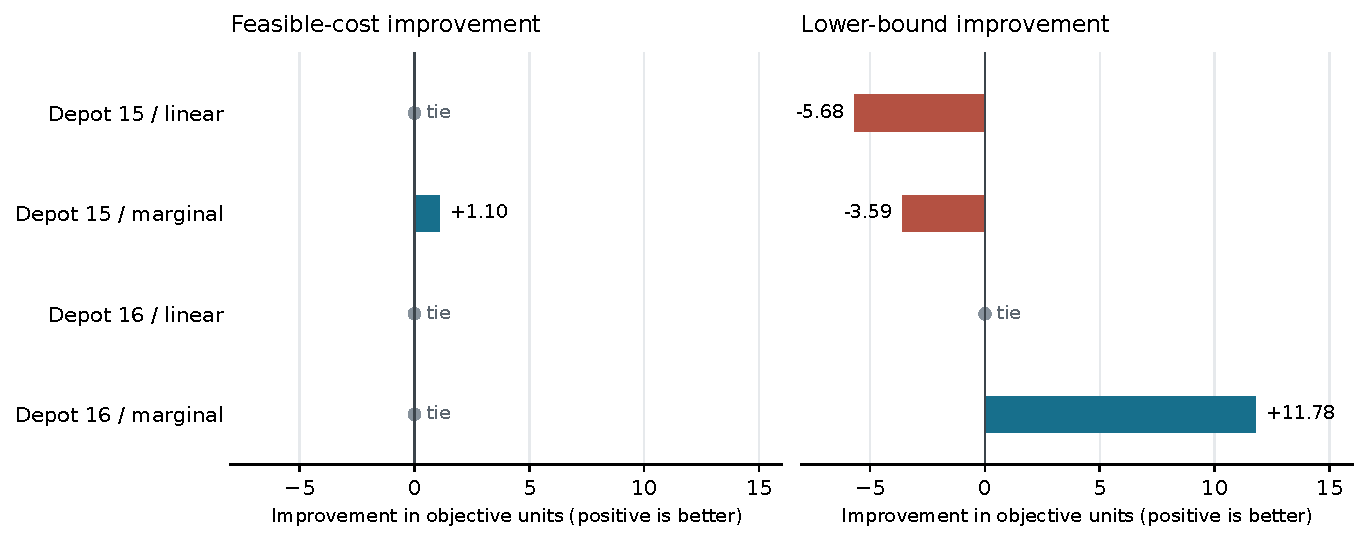
\includegraphics[width=\linewidth]{figures/pricing_start_effects.pdf}
\caption{Within-pair public effects of a submitted movement start on replayed incumbent and admitted lower bound at fixed native caps.  A smaller incumbent and a larger lower bound are favorable; the effects differ by query and depot.}\label{fig:pricing-start}
\end{figure}

The historical construction of the four shared source pools cost $358.21$~s once.  The preparation command, including source admission, cost a further $1.96$~s.  The 16 complete child receipts sum to $1{,}317.51$~s; adding the once-paid source work and freeze command gives $1{,}677.67$~s for this source-inclusive accounting.  Nested native, setup, and child timings must not be added again.  The source schedule was only modestly worse than the best newly returned public incumbent at this cap, with excess ranging from $0.32\%$ to $2.74\%$ of that returned incumbent's fixed-price objective.  This denominator is a feasible result, not the unknown fixed-price optimum.  No time to first incumbent was recorded, so the observed equal-cap quality cannot be converted into a start-induced time-to-solution claim.

\subsection{What the experiments establish}

\begin{table}[t]
\centering\small
\caption{Evidence map for the computational claims.  ``Established'' refers to the declared development cells and native-tolerance-qualified intervals, not to independent statistical replication.}\label{tab:computational-evidence-map}
\begin{tabular}{>{\raggedright\arraybackslash}p{0.30\linewidth}>{\raggedright\arraybackslash}p{0.60\linewidth}}
\toprule
Established in these cells & Still untested or unresolved \\
\midrule
Complete-fleet feasible columns can be reused across the two markets, and the multivisit target enclosure closed under reuse. & Whether reuse improves target-market global gaps or paid time across independent public timetables at equal quality. \\
Checked inherited physical-pricing evidence strengthened the selected lower in two completed public cached runs. & A causal cache effect against a completed, equally budgeted QP-without-cache target and a public global certification. \\
Movement starts were submitted and public fixed-price calls returned mixed incumbent/lower effects at equal native caps. & Native hint acceptance, time to first incumbent, and any robust start-induced speedup or learned-proposal benefit. \\
\bottomrule
\end{tabular}
\end{table}

The open public global intervals therefore remain the central computational limit for price support: a nearly solved restricted pool does not determine the full fleet hull or certify a target-market tariff.  Nearest-neighbor retrieval and learned proposals remain untested here; evaluation across independent timetable groups is future work.
